\documentclass[twocolumn,preprintnumbers,amsmath,amssymb,superscriptaddress]{revtex4}
%\usepackage[pdftex]{graphicx}

\usepackage{amsmath,amsfonts,amssymb}
\usepackage[english]{babel}
\usepackage[latin1]{inputenc}
\usepackage[T1]{fontenc}
\usepackage{color}
\usepackage{float}
\usepackage{verbatim}
\usepackage{graphicx}
\usepackage{bm}
\usepackage{mathtools}
\usepackage{stmaryrd}
\usepackage{anyfontsize}

\usepackage[font={small}]{caption}
\usepackage{subcaption}
\captionsetup{compatibility=false}

%\usepackage{epstopdf}
%\usepackage{array}
%\usepackage{tabularx}
%\usepackage{multirow}
\usepackage{color}
%\usepackage{multibox}
%\usepackage{rotating}
%\usepackage{lineno}
%\usepackage[left]{lineno}
%\usepackage[comma,sort&compress]{natbib}
%\usepackage{authblk}
%\usepackage{multicol}

\bibliographystyle{ieeetr}

\usepackage{bibunits}


%\linenumbers
%\setlength\linenumbersep{3pt}

\begin{document}


%\title{Simple rules yield complex communities: deconstructed species interactions and the assembly of communities}
%\title{Community assembly and dynamics by the deconstruction of species interactions}
\title{Lost in space: the eco-evolutionary impacts of straying on metapopulation persistence}
\author{Justin D. Yeakel${}^{1,2,*}$, Jean Phillipe Gibert${}^{1}$, Sean Anderson${}^{3}$, Peter Westley${}^{4}$, \& Jon W. Moore${}^{5}$ \\
${}^1$School of Natural Sciences, University of California, Merced, Merced CA, USA \\
${}^2$The Santa Fe Institute, Santa Fe NM, USA \\
${}^3$Department of Biology, University of Washington, Seattle WA, USA \\
${}^4$Institute for Arctic Biology, University of Alaska, Fairbanks, Fairbanks AK, USA \\
${}^5$Earth${}_2$Oceans Research Group, Simon Fraser University, Vancouver BC, Canada \\
${}^*$To whom correspondence should be addressed: jdyeakel@gmail.com
}



\maketitle



\section{Introduction}


%Motivation: straying
Coordinated mass migrations are one of the great wonders of the natural world, and the ability of individuals and groups to navigate across great distances have long fascinated naturalists \cite{MilnerGulland:2011vm}.
Anadromous salmonid fishes (genera \emph{Oncorhynchus} and \emph{Salmo}) embody these astonishing migrations by homing with high accuracy and precision to their natal streams for reproduction after years at sea \cite{Quinn:2011tf,Jonsson:2011kg,Keefer:2014gg}.
Nothwithstanding their philopatric tendancy, not all individuals home, but rather `stray' to non-natal sites to spawn \cite{Quinn:1993ge,Hendry:2004wf,H:2013fs}.
Although extensive work has been done to document the extent of straying from donor populations and into recipient populations \cite{Keefer:2014gg,Bett:2017ha}, only recently have the abiotic, biotic, and anthropogenic influences of `straying' behaviors been investigated systemically \cite{Keefer:2008bs,Westley:2015to,Bond:2016dz}.
Most recently the role of social interactions and collective navigation has been hypothesized \cite[][; this volume]{Berdahl:2015kv,Berdahl:2016dx}.
Although the straying of individuals into sites hosting other populations provides connections within the larger metapopulation, potentially promoting ecological and evolutionary rescue, it also serves to introduce maladapted individuals into habitats that are host to different environmental conditions, and this may lower the mean fitness of the local (mixed) population \cite{Muhlfeld:2014hs}.



%The tradeoff
The dual nature of straying as both promoter of connections among metapopulation demes and potential eroder of locally adapted gene complexes highlights the interplay between ecological dynamics of connected populations as well as the evolutionary dynamics of mixed trait distributions that respond to alternative local conditions.
Population-level biodiversity is recognized to increase species persistence (REFS), and the resilience and sustainability of metapopulations (general REF).
For example, the long-term sustainability of the Bristol Bay sockeye salmon fishery is due in large part to intact habitat that in conjunction with fine-scale homing and reduced gene flow provides a template for the evolution of countless locally adapted populations \cite{Hilborn:2003gf,Schindler:2010he,Anonymous:2014ku,Satterthwaite:2015ge}.
In contrast, areas such as California's Central Valley where habitats have been lost, degraded, and homogenized stand in marked contrast.
Within species diversity (or lack thereof) can manifest itself by way of asynchronous population dynamics, where the drivers that give rise to changes in population size vary across a metapopulation, decreasing the potential for synchronization, and correspondingly increasing the potential for ecological rescue (REFS).
This statistical buffer against extinction has traditionally been quantified as the Portfolio Effect (PE), which is the ratio of the population CV to the CV of the aggregated metapopulation.
Weakened portfolio dynamics can also emerge from homogenization resulting from  reduced genetic variability among populations, where homogenous stocks are more likely to have similar life-history structures (REFS), be at greater risk disease-induced epidemics (REFS), and recruit sub-optimally in heterogeneous environments (REFS).
Of course, these two measures of diversity often occur concurrently: for instance, lower genetic diversity increases the likelihood that two populations respond similarly to the same stressors, and this promotes synchronized dynamics, thus lowering portfolio effects.

%Eco-evolutionary dynamics in space
%% From geographic mosaic of coevolution to...
That evolutionary forces play out heterogeneously across geographic mosaics is now a foundational concept in ecology and evolutionary biology (REFS).
These mosaics are in part driven by environmental differences between habitats that alter the selective forces acting on different phenotypes \cite{Endler:1986tz}, and a principle underlying assumption is that there is gene flow such that individuals from different habitats mix over space (REFS).
Although the evolutionary outcomes of these spatial processes have been explored in depth (REFS), it is less well understood how selective mosaics and their consequent evolutionary forces impact population dynamics over contemporary timescales \cite{Hendry:2016un}.
How the ecological dynamics of phenotypically diverse metapopulations, wherein constituent populations are subject to different selective regimes, are altered affected by evolutionary forces is less well known. % and the subject of this paper.

%Movement through space (link back to straying)
Migratory populations that return to a breeding ground or natal stream to reproduce are linked to each other by some proportion of the population that permanently disperse, or stray into the `wrong' site; we might say that there is at least one \emph{Kevin} in every school or flock in every school or flock (Fig. \ref{fig:xkcd}).
The rate at which individuals stray, $m$, has been subject to a growing amount of both theoretical and empirical research \cite{H:2013fs,Keefer:2014gg,Bett:2017ha} and may be linked to errors made at an individual-level that are themselves diminished by migrating in groups and pooling individual choices \cite{Berdahl:2015kv,Berdahl:2016dx}.
Regardless of the mechanism's governing straying, the effect that it has on the dynamics of individual populations and the metapopulation as a whole is a topic of considerable interest that has tangible conservation implications \cite{Brenner:2012gl,Johnson:2012fe,Fullerton:2011ii}.
Whether, and to what extent, the ecological consequences of straying depend on the evolutionary dynamics that emerge from populations distributed across a selection mosaic is unclear.
How the assumed negative evolutionary effects of straying and subsequent gene flow is balanced by the positive effects of demographic rescue is the subject of this contribution.

%Here we show: pattern formation, dependence on heritability, large effects of small amounts of straying

\begin{figure}
  \captionsetup{justification=raggedright,
singlelinecheck=false
}
\centering
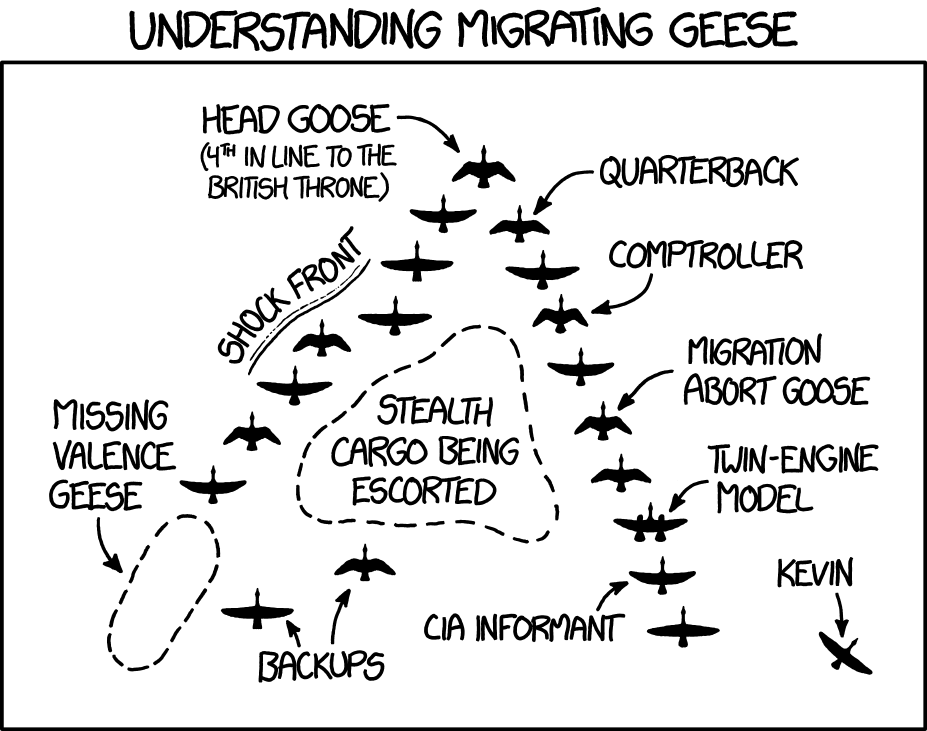
\includegraphics[width=0.4\textwidth]{figs2/fig_xkcd.png}
\caption{
\emph{Migrating Geese}, a comic from Randall Monroe's xkcd (https://xkcd.com/1729/). 
A flock of geese travel in the direction of a shared destination, the lone stray named \emph{Kevin}.
In this case, the rate of straying is $m=0.05$, which is not an uncommon rate for migrating populations of salmon \cite{Satterthwaite:2015ge}. 
Reprinted under the Creative Commons Attribution-NonCommercial 2.5 License.
} \label{fig:xkcd}
\end{figure}

%Alternative stable state
Here we ask the overarching question of how collective behavior mediated dispersal and gene flow interact to influence the persistence of locally adapted populations and persistence of those populations.
To address this question we construct a minimal eco-evolutionary model of two populations occupying different sites that are linked by straying individuals, each of which with an associated trait distribution subject to natural selection determined by local conditions.
An important and relatively novel component of this model is the inclusion of a parameter that defines the difference in local conditions that favor different trait optima, increasing values of which correlates to populations that mix across increasingly heterogeneous environments \cite[though see ]{Berdahl:2015kv}.
Although our proposed model is was constructed with the dynamics of salmon populations in mind, the framework is general and the conclusions are likely relevant to a diverse range of migratory organisms where locally adapted populations are linked by dispersal.
We first show that specific rates of straying and trait heritability can have large effects on the qualitative dynamics of populations over time, in many cases giving rise to alternative steady states where one site is pushed towards very low biomass.
The emergence of alternative steady states results in a nonlinear response of the portfolio effect, suggesting that metapopulation persistence can be quite sensitive to the combined influences of collective straying across a selective landscape.

%Extinction and return times

%Habitat heterogeneity
A second important finding of our minimal model reveals that systems with greater habitat heterogeneity (measured by an increased difference in the trait values that are optimal between sites) host an intermediate range of straying rates where the portfolio effect increases to a local maximum, signaling that under certain conditions moderate amounts of straying between populations can increase the likelihood of persistence despite the deleterious evolutionary effects overall.
However, if we suppose that the rate of straying between two sites is correlated with distance (as indicated by empirical evidence), and that the difference in trait optima increases with distance as would be the case if the optima were associated with alternative temperature regimes (especially if sites are distributed latitudinally rather than longitudinally), even a very small amount of straying can drastically reduce the portfolio effect.
Importantly, the qualitative nature of our results do not depend on whether the stray rate is density dependent or constant, suggesting a limited role of collective dispersal on the dynamics considered herein.

%Concluding paragraph of the intro




\section{Model Description}

\noindent{\bf (a) Metapopulation framework}\\
\noindent Here we consider two populations $N_1$ and $N_2$ that are separated in space in distinct habitats, each with trait values $x_1$ and $x_2$ determining recruitment rates.
We assume that there is an optimum trait value $\theta_1$ and $\theta_2$ associated with each habitat, where recruitment is maximized if the trait value of the local population $x = \theta$.
Moreover, we assume that $x_{1,2}$ are normally distributed with means $\mu_1$ and $\mu_2$ and have a shared standard deviation $\sigma$.
As such, the recruitment rate for both populations is determined by the mean trait value of the local population, such that $r_1 = R_1[\mu_1(t)|\theta_1]$.
Trait means for each population are subject to selection, the strength of which depends on the difference between the population mean and the local trait optimum at a given point in time \cite{simpson1953major,Lande:1976ga}.

The two populations are assumed to reproduce in spatially separate sites that are close enough such that a proportion of the population $m$ can stray into the other site, and where mortality occurs before individuals return to reproduce.
If there is no straying between these populations (such that they are independent), then the mean trait evolves towards the optimal value such that $x_1 \rightarrow \theta_1$, and the recruitment rate for that population will be maximized.
If there is straying between populations at rate $m$, then the traits in each respective location will be pulled away from the optimum, and recruitment rates will be lowered.
As $m \rightarrow 0.5$, the populations are perfectly mixed, acting as a single population.

\begin{figure}
  \captionsetup{justification=raggedright,
singlelinecheck=false
}
\centering
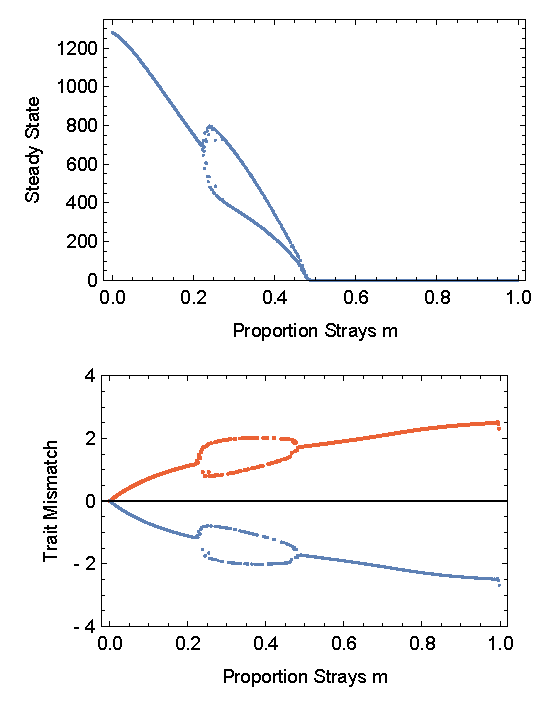
\includegraphics[width=0.4\textwidth]{figs2/fig_Density.pdf}
\caption{
A) The steady state densities of $N_1$ and $N_2$ as a function of a constant stray rate $m$.
B) The steady state trait values measured as $\theta_i - x_i$, as a function of a constant stray rate $m$. 
} \label{fig:traj}
\end{figure}

We use the discrete Ricker population dynamic framework described by Shelton and Mangel \cite{Shelton:2011eq} as the basis for our two-site model, with the added effect of the local population $N_i$ mixing with a set proportion $m$ of a remote population $N_j$ that is straying into it.
We first assume that the proportion ${\rm e}^{-Z}$ of both populations survive, and that the aggregated mix of the populations (local individuals in addition to the straying individuals) are subject to the same compensatory effects, determined by the parameter $\beta$.
For a local site $i\in(1,2)$ that collects straying individuals from a remote site $j\in(1,2)$, if $N_i$ is the local site and $N_j$ is the remote site, the difference equation that determine changes in population size is

\begin{align}
  &N_i(t+1) = \\ \nonumber
  &\left((1-m)N_i(t) + m N_j(t) \right){\rm e}^{-Z} \\ \nonumber
  &+ \left(R_i[\mu_i(t)] (1-m)N_i(t) + R_i[\mu_j(t)] m N_j(t)\right) \\ \nonumber
  &\times {\rm e}^{-\beta ((1-m)N_i(t) + m N_j(t))},
  \label{eq:N}
\end{align}

\noindent where a small amount of demographic process error is added to the reproductive rate, and where the difference equation for $N_j$ mirrors that for $N_i$.

The combined recruitment of local individuals $(1-m)N_i(t)$ and incoming strays $mN_j(t)$, as a function of their mean trait value at time $t$ and given the local trait optimum $\theta_i$, is then

\begin{align}
  &R_i[\mu_i(t)] = \\ \nonumber
  &\int_{-\infty}^\infty r_{\rm max}\exp\left\{\frac{(x_i(t)-\theta_i)^2}{2\tau^2}\right\} {\rm pr}(x_i(t)|\mu_i,\sigma^2) {\rm d}x_i(t) +\tilde{P}\\ \nonumber
  &= \frac{r_{\rm max} \tau  }{\sqrt{\sigma ^2+\tau ^2}}\exp\left\{-\frac{(\theta_i-\mu_i(t))^2}{2 \left(\sigma ^2+\tau ^2\right)}\right\} +\tilde{P},
  \label{eq:R}
\end{align}

\noindent where the mismatch between the local trait mean $\mu_i(t)$ and the local optimum $\theta_i$ determines the recruitment rate for the population, and $\tilde{P}$ introduces a small amount of demographic error $\tilde{P}\sim {\rm Normal}(0,0.01)$.
The parameter $\tau$ controls the sensitivity of recruitment to changes in the mean trait value away from the optimum, which we set as $\tau=1$ here and throughout.
% The compensatory effects are then determined by the exponential, following the Ricker stock-recruitment relationship.
\\

\begin{figure*}
  \captionsetup{justification=raggedright,
singlelinecheck=false
}
\centering
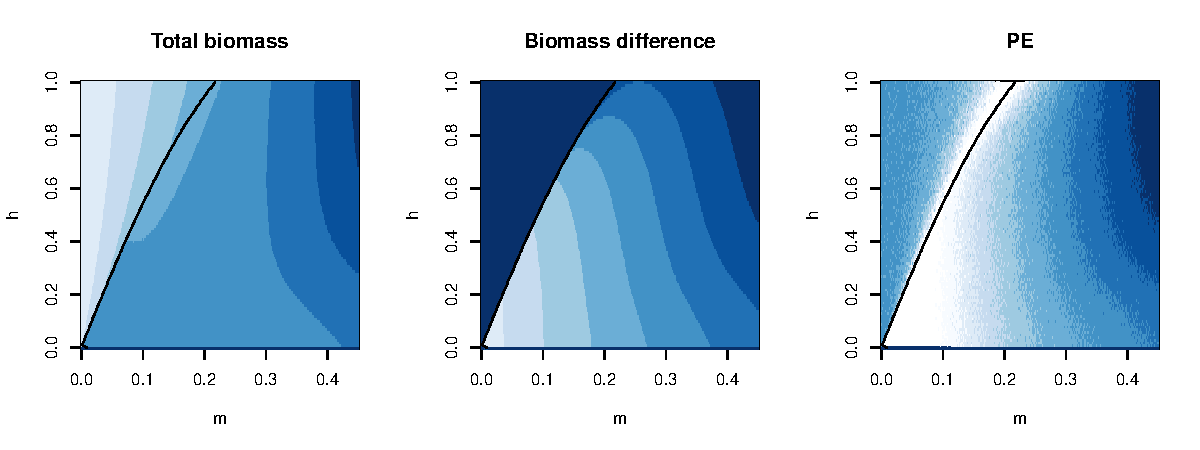
\includegraphics[width=0.8\textwidth]{figs2/fig_MDPE_hm.pdf}
\caption{
(a) Total means $N_t$, (b) difference in means $\Delta N$, and (c) the portfolio effect PE as a function of heritability $h^2$ and a constant stray rate $m$. Light colors = high values.
The black line shows the fold bifurcation separating a single steady state (left) from alternative steady states (right).
(d) The relationship between the time to recovery following a disturbance and the portfolio effect.
} \label{fig:PE}
\end{figure*}

\noindent{\bf (b) Recruitment over a selective landscape}
\noindent Because individuals from the local population are mixed with individuals from the remote population via staying, the resulting trait distribution is a mixed normal with weights corresponding to the proportion of the mixed population that are local individuals, $w_i$, and for the straying individuals, $1-w_i$, where 
\begin{equation}
w_i=\frac{(1-m)N_i(t)}{(1-m) N_i(t) + m N_j(t)}.
\end{equation}
We make two simplifying assumptions.
First, we assume that the distribution resulting from the mix of remote and local individuals, following reproduction, is also normal with a mean value being that of the mixed-normal.
Second, we assume that changes in trait variance through time are minimal, such that $\sigma$ is assumed to be constant.



An increasing flow of incoming strays is generally expected to pull the mean trait value of the local population away from its optimum over time, which will decrease its rate of recruitment.
The mean trait value thus changes through time according to the difference equation

\begin{align}
  \mu_i(t+1) &= w_i\mu_i(t) + (1-w_i)\mu_j(t) \\ \nonumber
  &+ h^2\sigma^2\frac{\partial}{\partial \mu_i}\ln\left(w_i R_i[\mu_i(t)|\theta_i] + (1-w_i)R_i[\mu_j(t)|\theta_i]  \right),
  \label{eq:mu}
\end{align}

\noindent where the first two factors determine the mixed normal average of the now-mixed local and remote populations.
This mixed normal is weighted by the proportion of the population that is local and remote, respectively, which depends on the stray rate $m$.
The partial derivative in the Eq. \ref{eq:mu} determines how the mean trait changes through time due to natural selection (REF), which is proportional to the change in mean fitness with respect to $\mu_i$.
\\

\noindent {\bf (c) Measuring metapopulation persistence}
\noindent We evaluated metapopulation persistence by measuring the average-CV portfolio effect (PE) (REF: Anderson,others) as well as the time required for the system to return to a steady state following an induced disturbance to one or both of the populations.
The average-CV portfolio effect is, as the name implies, the average CV across each population divided by the CV of the aggregate, such that


\begin{equation}
\langle{\rm PE}\rangle =\frac{1}{X}\sum_{i=1}^{X} \frac{\sqrt{{\rm VAR}(N_i)}}{{\rm E}(N_i)}\cdot \frac{{\rm E}(N_T)}{\sqrt{{\rm VAR}(N_T)}},
\label{eq:pe}
\end{equation}

\noindent where in this case the number of populations is limited to $X=2$ and the expectations $\rm E(\cdot)$ and variances $\rm VAR(\cdot)$ are evaluated at the steady state.
As the CV of $N_T$ decreases relative to that of the constituent populations, $\langle{\rm PE}\rangle > 1$, and the metapopulation is presumed to become more stable.
A similar measure of metapopulation persistence can be evaluated by measuring the synchronization $\phi$ between populations, where 
\begin{equation}
\label{eq_sync}
\phi = \frac{{\rm VAR}(N_T)}{\left(\sum_{i=1}^N\sqrt{{\rm VAR}(N_i)}\right)^2}.
\end{equation}
By rearranging and substituting eq. (\ref{eq_sync}) into eq. (\ref{eq_PE}), we can observe that $\langle{\rm PE}\rangle \propto \sqrt{\phi}^{-1}$.
Thus, the dynamical diversity of the metapopulation offers a mirror to the portfolio effect, where perfect synchrony ($\phi = 1$) also means $\langle{\rm PE}\rangle = 1$.
%Moreover, if and only if $\phi \neq 1$, it is expected that as the diversity of the aggregate increases, so should the portfolio effect, and this central thesis is thought to underlie the stability of populations, species, communities and even financial markets.
Portfolio effects greater than unity corresponds to less synchronization ($\phi < 1$) \cite{Loreau:2008ju,Anderson:2014cx,Yeakel:2013vz} and thus a greater potential for demographic rescue among populations, buffering the system as a whole against extinction. 

%Although there are more robust ways to measure the portfolio effect (in particular for comparing the PE across species with different mean-variance relationships; REF: Anderson), its only utlity here is to provide a simple statistical measure of metapopulation persistence.
A more direct way to measure system persistence is to measure the time that it takes it to relax back to its steady state following an induced disturbance: systems that recover quickly (shorter recovery times) are more robust than those that recover more slowly (longer recovery times).
Measuring the time that it takes for a perturbed system to relax also permits a more detailed perspective of the potential fragility of the metapopulation.
For example, if populations settle to alternative steady states (alternative steady states in our model requiring one population to be high-density and one low-density), comparing recovery times after a disturbance applied to the high, low, and/or both populations allows for an assessment of which component of the metapopulation has a longer-lasting influence on the system's recovery.
\\

\noindent {\bf (d) The effects of density and distance on the rate of straying}
%Density dependent m
\noindent We have so far assumed that the proportion of strays leaving and entering a population is constant, however there is good evidence that at least in some species the straying rate is density dependent (REFS).
Specifically, the rate at which individuals stray has been linked directly to a collective decision-making phenomenon, where greater numbers of individuals tend to decrease the rate at which individuals err, reducing the overall proportion of a population that strays.
According to Berdahl et al. \cite{Berdahl:2016dx}, given the probability that an individual strays is $m_0$, the proportion of the local population $N_i(t)$ that strays is

\begin{equation}
  m(t) = m_0\left(1- \frac{N_i(t)}{C+N_i(t)}\right),
  \label{eq:ddm}
\end{equation}

\noindent where $C$ is a half-saturation constant.
We note that at the limit $C\rightarrow \infty$, the density dependent stray rate becomes constant such that $m(t) \rightarrow m_0$, and this corresponds to the original formulation where $m=m_0$.
A similar observation shows that when the population density is very high, $m(t) \rightarrow 0$, and when it is close to extinction, $m(t) \rightarrow m_0$.
Thus, for realistic population densities, $m(t) < m_0$.


%Linking m/m0 and thetadiff
The straying rate is intrinsically linked to the distance between the donor and recipient population.
The greater the distance between two populations, the lower the expected rate of straying (REF).
We can account for this interdependence in our model by assuming that $m$ (if the stray rate is constant) or $m_0$ (if the stray rate is density dependent) is a function of the difference between optimal trait values between sites $\theta_i-\theta_j$, which can be assumed to be large if the remote site $j$ is a great distance away from the local site $i$.
If sites $i$ and $j$ are very close, the stray rate is maximized at $m,m_0 = 0.5$, assuming both sites are equally attractive to the respective populations.
Thus, we can integrate these two variables by setting $m,m_0 = (2 + \epsilon (\theta_i-\theta_j))^{-1}$, where $\epsilon$ sets the sensitivity of a declining $m$ to increasing distance (greater values of $\theta_i-\theta_j$).

\begin{figure*}
  \captionsetup{justification=raggedright,
singlelinecheck=false
}
\centering
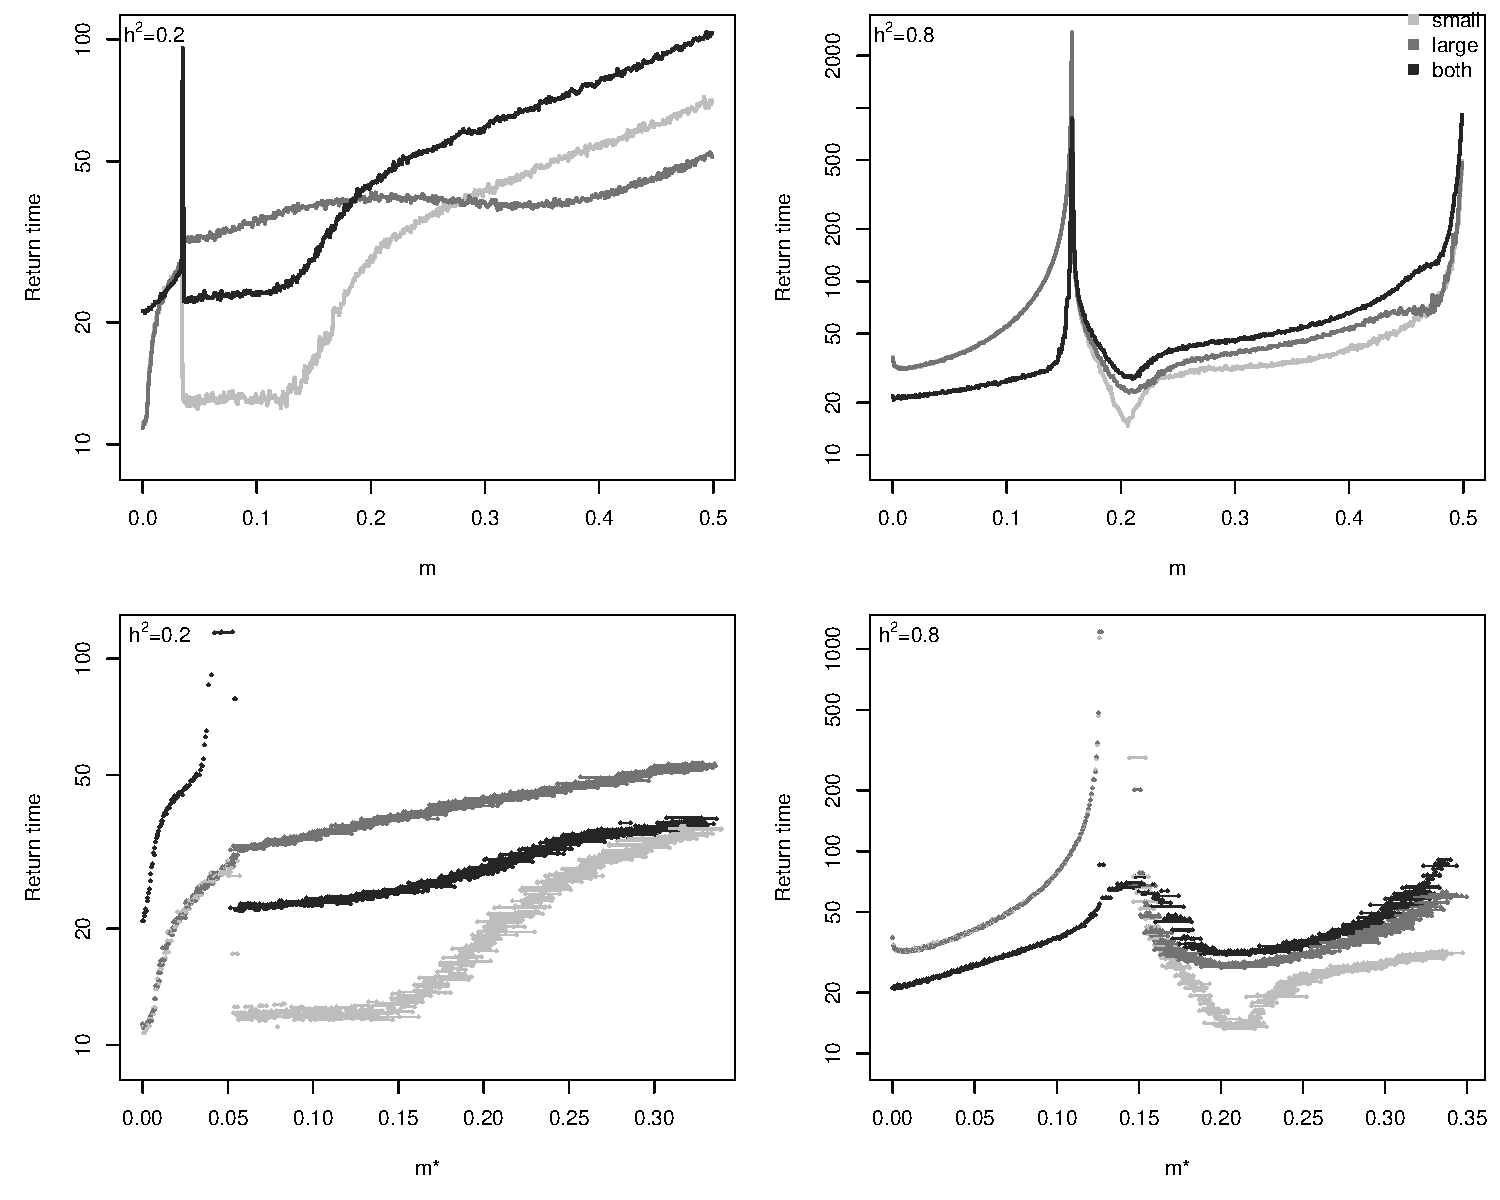
\includegraphics[width=0.9\textwidth]{figs2/fig_relax_comb.pdf}
\caption{
Top row (a, b)
Bottom row (c, d)
} \label{fig:relax}
\end{figure*}



\section{Results}

%The effects of trait evolution :: trait heritability, trait variance, and habitat heterogeneity
%% Bifurcation to alternative stable state occurs at higher stray rates with increased trait heritability
%% There is a peak in the portfolio effect directly before this bifurcation is crossed (early warning signal), and then a decline in PE with high m
%% When trait heritability is high, there is a greater sensitivity of total biomass to increasing stray rates, though a LOWER sensitivity of the difference between alternative steady state values for increasing stray rates (and vice versa)
%% For low heritability (h = 0.01 - 0.2 or so), moderate and insensitive changes in total biomass, but large differences between the values of alternative steady states leads to a local maximum for PE at low-moderate stray rates



%Alternative stable states

\noindent{\bf (a) Nonlinear effects of straying on the portfolio effect and recovery time} \\
\noindent Straying generally lowers steady state densities for both recipient and donor populations by \emph{i}) losing locally-adapted individuals to the non-local population and \emph{ii}) gaining maladapted individuals from that same population. %, regardless of trait heritability and variance or habitat heterogeneity
The decline in steady state densities is not gradual: as straying increases, the system crosses a fold bifurcation whereby the single steady state across both sites bifurcates into two alternative steady states: one at high biomass density, and one at low biomass density (Fig. \ref{fig:traj}a,b).
This bifurcation  (shown by the black line in Fig\ref{fig:PE}(a-c)) occurs at lower values of the straying rate $m$ at lower values of trait heritability $h^2$ (Fig \ref{fig:PE}a,b), indicating that weaker coupling between ecological and evolutionary dynamics in addition to higher rates of straying promotes the appearance of alternative stable states.

Trait heritability has a large impact on the sensitivity of the straying rate to both the aggregate population steady state density ($N^*_T=N^*_1+N^*_2$; Fig. \ref{fig:PE}a) as well as the difference between steady state densities (the distance between alternative stable states: $\Delta N=|N^*_1-N^*_2|$; Fig. \ref{fig:PE}b).
Greater trait heritability results in a larger decline in $N_T^*$ for increasing straying rates $m$, but leads to only moderate changes to $\Delta N$.
Conversely, if the trait is less heritable, an increase in the straying rate has little impact on the total biomass density but contrastingly large effects on $\Delta N$.




%Together these changes in steady state population densities in terms of $N_T$ and $\Delta N$ as a function of trait heritability and the rate of straying between populations give rise to highly nonlinear portfolio effects, which we quantify here as

% Nonlinear PE(!!!)

%In the region where there is a single steady state among both populations, we find an low-intermediate portfolio effect ca. ${\rm PE}=1.4$, primarily due to the elevated mean values of $N_T$.
As the fold bifurcation is reached with greater rates of straying, the portfolio effect increases sharply due to an explosion in variance of both donor and recipient populations ${\rm VAR}(N_{i,j})$.
This increase in variance is the product of a dynamical process known as critical slowing down that occurs near fold bifurcations \cite{Scheffer:2009gg}, and may serve as an early warning signal of an approaching phase transition \cite{Scheffer:2009gg,Anonymous:2013br,Dakos:2014br}.
For larger values of $m$ (to the right of the fold bifurcation in Fig \ref{fig:PE}(a-c)), where alternative steady states occur, the portfolio effect declines steadily as the CV of $N_T$ increases.
The decline over $m$ is more gradual if trait heritability is low, and steeper if trait heritability is high.



% \noindent{\bf (c) Rates of recovery following catastrophic collapse}\\ 
% Return time as a measure of system persistence and relation to PE
We measured the time required for the system as measured by $N_T$ to relax to its steady state as a function of straying rate following three types of induced disturbance: (\emph{i}) extinction of the low-density population; (\emph{ii}) extinction of the high-density population (scenarios \emph{i} and \emph{ii} amount to the same in the single steady state regime); (\emph{iii}) near-collapse of both populations where just 1.0\% of both populations survive.
In general, the average-CV portfolio effect is negatively correlated with recovery time (Fig. \ref{fig:PE}d), suggesting that for our system both measures are valuable indicators of metapopulation persistence.
Because we can assess the time to recovery in response to the various disturbance types described above, it allows us to gain an in-depth perspective on the fragility of the metapopulation as a function of straying rate.

At low rates of straying both populations are subject to the same steady state, such that extinction of either population results in the same recovery time.
At low rates of straying and low trait heritability, the time required to recover following the extinction of either population is generally less than or equal to the recovery time required after the near-collapse of both populations (Fig. \ref{fig:relax}a).
In the alternative stable state regime, extinction of the smaller population results in the shortest recovery time, whereas as $m$ increases, extinction of the larger population results in the shortest recovery time.
Increased trait heritability flips this picture around (Fig. \ref{fig:relax}b).


If both straying rate and heritability are low, extinction of the small population results in shorter recovery times, whereas for higher straying rates, the extinction of the larger population results in shorter recovery times.
This switch is in part due to a large burst in biomass of the surviving (large) population when the smaller of the two becomes extinct at high straying rates, which extends the time required for the smaller population to recover.
Conversely, with increased trait heritability (Fig. \ref{fig:relax}b) and low straying rates in the single steady state regime, near collapse of both populations (rather than the extinction of either) results in the lowest recovery time.
Near the onset of the fold bifurcations, recovery times increase drastically, regardless of disturbance.
For straying rates in the alternative steady state regime, extinction of the smaller population consistently results in the shortest time to recovery.


\begin{figure}
  \captionsetup{justification=raggedright,
singlelinecheck=false
}
\centering
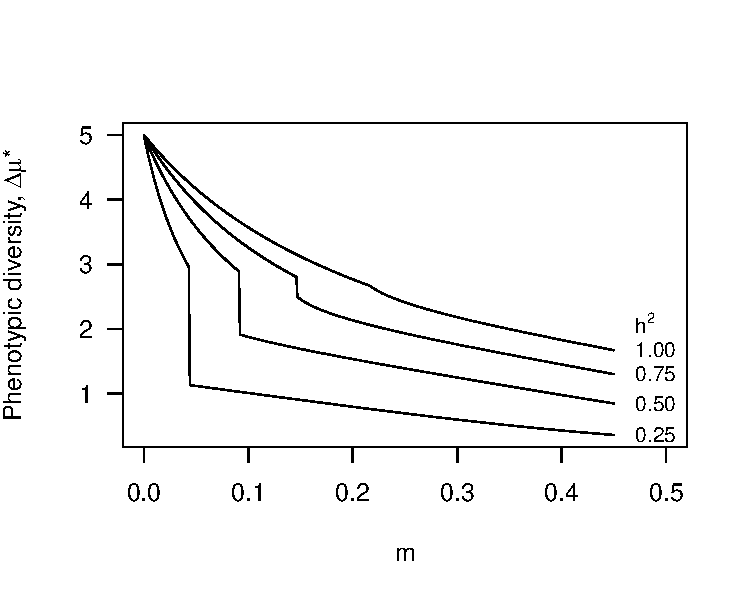
\includegraphics[width=0.5\textwidth]{figs2/fig_traitdiff.pdf}
\caption{
Phenotypic diversity ($\Delta \mu$) evaluated at the steady state as a function of straying rate $m$ and trait heritability $h^2$. The descrete jump occurs as the system crosses the fold bifurcation; lower phenoytic diversity emerges with higher straying rates and in the alternative steady state regime. 
} \label{fig:traitdiff}
\end{figure}

%Lowering Phenotypic diversity with increasing straying rate
Increased rates of straying lowers phenotypic diversity ($\Delta \mu = |\mu_i(t)-\mu_j(t)|$, evaluated at the steady state) because both local and remote populations are increasingly homogenized.
The sensitivity of this phenotypic homogenization to straying is increased with lower heritability because the selective forces acting against trait means far from the local optima are lessened for lower $h^2$.
Less intuitively, we observe a discrete jump towards low phenotypic diversity at low-moderate ($0.05 \leq m < 0.2$) straying rates, which occurs as the consequence of crossing the fold bifurcation (Fig. \ref{fig:traitdiff}).
Although the development of alternative stable states elevates the portfolio effect due to the variance-dampening effects of the aggregate, this change in dynamic regimes is also associated with a substantial decline in phenotypic diversity. 
\\

\begin{figure}
  \captionsetup{justification=raggedright,
singlelinecheck=false
}
\centering
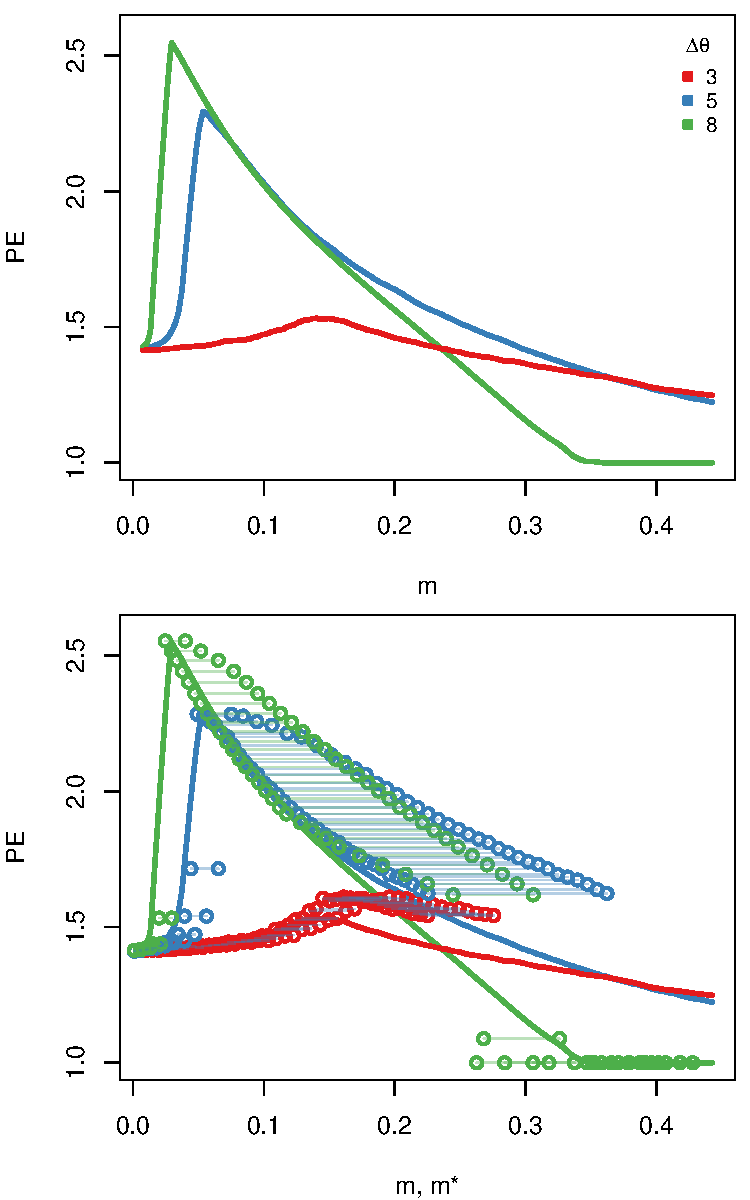
\includegraphics[width=0.4\textwidth]{figs2/fig_thetaPEmvm.pdf}
\caption{
(a) Median portfolio effect as a function of stray rate $m$ for lower trait heritability ($h^2 < 0.5$).
Vertical dashed lines represent the fold bifurcation, which occurs at lower stray rates with increased habitat heterogeneity $\Delta \theta$.
(b) Within the box shown in (a), PE as a function of the constant straying rate is shown as the solid line. Paired open circles show PE as a function of a density dependent straying rate. Straying rates are paired because the recipient and donor populations exist in alternative steady states. The lower straying rate of a pair is for the larger population; the higher straying rate is for the smaller population.
The different steady state regimes that give rise to the range of straying rates were obtained by varying the individual straying probability $m_0$ (where $m_0$ and $m^*$ are linearly related).
} \label{fig:thetaPE}
\end{figure}

%% Increased habitat heterogeneity
  %%% 1) exaggerates lowering of mean biomass with increasing stray rates
  %%% 2) increases the likelihood of alternative stable sites & increases the differences in alternative stable state values with increasing stray rates
  %%% 3) decreases the PE (!!)

\noindent{\bf (b) The role of habitat heterogeneity on the portfolio effect}\\ 
\noindent Increased differences in optimal trait values between sites ($\Delta\theta = \left|\theta_i - \theta_j\right|$) corresponds to greater between-site differences in conditions that favor alternative traits, interpreted here as increased habitat heterogeneity.
At one end of the spectrum, if both populations are isolated, natural selection would direct the mean trait values of both populations towards their respective optima, such that $\mu_i(t) \rightarrow \theta_i$ as $t\rightarrow\infty$.
%difference in optimal trait values between the local and remote populations, which we call .
However when straying exists, we find that increasingly divergent trait optima generally lowers $N_T$ and exaggerates $\Delta N$, such that one population has the majority of the biomass (Appendix Fig. \ref{fig:thetadiff1},\ref{thetadiff2}).
Which population becomes large or small depends on the initial conditions, which are randomized. 
The impact of habitat heterogeneity on the portfolio effect is more complex, serving to emphasize the nonlinear relationship between the stray rate and the PE, regardless of heritability.
%The rate of straying that gives rise to a large PE at the fold bifurcation is conditioned on the difference in optimal trait values between the local and remote populations, which we call $\Delta\theta = \sqrt{(\theta_i - \theta_j)^2}$.
The extent of the nonlinearity between $m$ and the PE depends very much on $\Delta\theta$, particularly when trait heritability is low ($h^2<0.5$).
As habitat heterogeneity increases, the fold bifurcation and associated spike in PE generally occurs for lower values of straying rate $m$, meaning that a lower amount of straying can give rise to alternative stable states (Fig. \ref{fig:thetaPE}).
In the region where alternative stable states are feasible (Fig. \ref{fig:thetaPE}), additional straying increases the portfolio effect to a local maximum before its negative effects serve to lower PE as $m\rightarrow 0.5$, and this effect is exaggerated with increasing habitat heterogeneity.
\\




% Density dependent m
%% Because m[t] @ steady state 0<m[t]<m0, we observe the same dynamics for higher m0 as we do for lower constant m.
%% Higher rates of straying are tolerable (there is a not a decline in PE for very high m0 as there is for constant m)

\noindent{\bf (c) The effects of density dependent straying}\\
\noindent If we assume that the rate of straying is density dependent, the probability of straying at the individual level $m_0$ determines the rate of straying within the population, such that $m(t)$ becomes lower as $N(t)$ increases (Eq. \ref{eq:ddm}).
At the steady state $m(t)=m^*$ is also constant, though by definition, it is always less than $m_0$ such that $0 < m^* < m_0$.
Because our analyses concern steady state conditions, the inclusion of density-dependent straying does not have a large impact on the qualitative nature of our findings (Appendix Fig. \ref{fig:ddm}).

The assumption that straying is density dependent alters the strength of the portfolio effect for a given $m^*$.
As shown in Figure \ref{fig:thetaPE}(b), in the alternative stable state regime, because the recipient and donor population exist at different steady state densities, they have different rates of straying such that a given value of the portfolio effect is now associated with a pair of straying rates $(m_i^*,m_j^*)$.
A range of $(m_i^*,m_j^*)$ values are obtained by varying $m_0$, which is positively and linearly related to $(m_i^*,m_j^*)$.
Importantly, we show that metapopulations settling at relatively low rates of straying have lower-than-expected portfolio effects, whereas metapopulations settling at relatively high rates of straying have higher-than expected portfolio effects.
This suggests that there is a strong tradeoff in the role of density dependent straying on the persistence of metapopulations: as the individual probability of straying is lowered, the straying rates of both recipient and donor populations are similarly lowered, however this diminishes the system's ability to buffer itself against extinction as measured by the portfolio effect.
Conversely, as the probability that an individual strays increases, so does rate of straying for both recipient and donor populations, and this serves to elevate the portfolio effect compared to a constant $m$.
This effect remains but is somewhat diminished as habitats become increasingly heterogeneous.

Return times (Fig. \ref{fig:relax}c,d).
\\

\begin{figure*}
  \captionsetup{justification=raggedright,
singlelinecheck=false
}
  \centering
  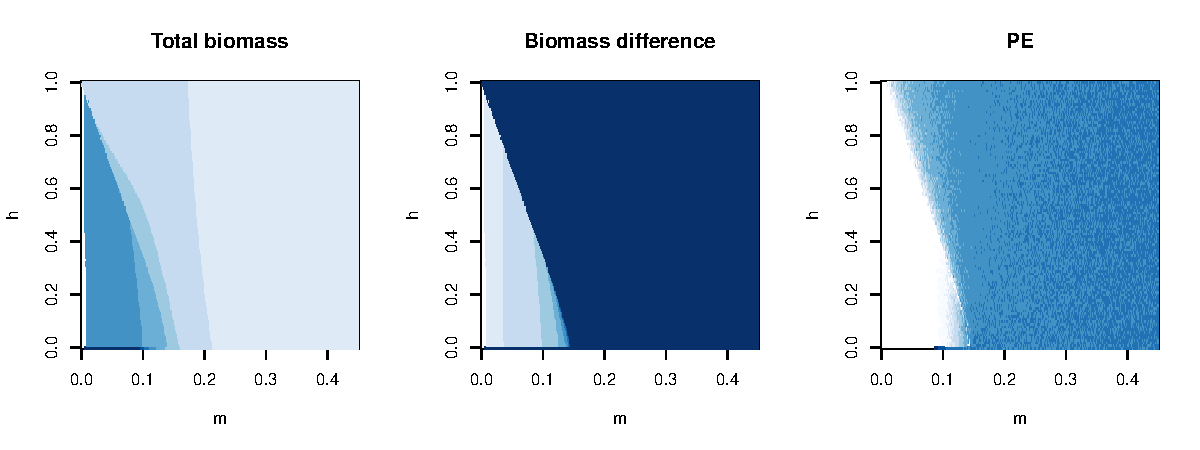
\includegraphics[width=0.8\textwidth]{figs2/fig_MDPE_hm_mtheta.pdf}
  \caption{
  Assuming that the rate of straying is linked directly to habitat heterogeneity. A low stray rate corresponds to very different (or distant) habitats (high $\Delta\theta$), whereas a higher rate of straying corresponds to very similar (or nearby) habitats (low $\Delta\theta$). Light colors = high values.
  } \label{fig:mtheta}
\end{figure*}


% When m and thetadiff are linked
%%Constant m
  %%% Low stray rate (high theta1-theta2) leads to alternative stable states and relatively low PE ~ sharp transition
  %%% High stray rate (low theta1-theta2) increases the steady state (and no A.S.S.)... 
  %%% This suggests that space naturally buffers against the negative effects of mixing dissimilar populations, however it is NOT SMOOTH
  %%% This is particularly true for low heritability. High heritability eliminates the A.S.S. region
  %%% (!!!) Even low levels of straying from distant populations can result in highly divergent alternative steady states! THIS IS A COOL RESULT

\noindent{\bf (d) Distance dependent straying and habitat heterogeneity}\\ 
\noindent We have so far treated $\Delta\theta$ and $m$ as independent parameters, however we may also assume that if environmental heterogeneity increases with distance, the rate of straying may be expected to decline given that individuals are less likely to stray into distant habitats. %-- in particular North-South difference if trait optimality is largely temperature-dependent --
If we incorporate this interdependence of $m$ and $\Delta\theta$, low rates of straying would correspond to mixing dissimilar (distant) populations, and high rates of straying would correspond to mixing similar (nearby) populations.

Here we find that alternative stable states now appear for low straying rates ($m<0.15$) and over any value of trait heritability $h^2<1$.
As the straying rate increases, a single stable state emerges with a correspondingly high $N_T$.
As before, there is a spike in the PE at the fold bifurcation separating the alternative stable state regime from the single stable state regime, and a sharp decline in the PE as the straying rate becomes very low.
This is in accordance with intuition as increasing straying rates mean that two very similar populations are mixing, such that the rate of recruitment is less influenced by gene flow.

That alternative stable states appear and that PE becomes severely depressed for very low rates of straying is surprising: this means that even a small amount of mixing of populations from distant or dissimilar populations can qualitatively alter the dynamics of the metapopulation, regardless of trait heritability.
%(for the discussion: an example of this situation may be the salmon populations during the last glacial maximum, where any mixing would be from geographically distant populations)



\section{Discussion}

We have shown that the natural selection of mixed populations adapted to different environments can result in large effects on population dynamics and the degree to which the metapopulation is buffered against extinction, quantified here as the portfolio effect.
The immigration of dispersing strays with trait values far from the local optimum generally lowers the combined steady state biomass $N_T$ and increases the likelihood that the system gives way to alternative steady states, pushing one of the populations close to extinction.
Although the emergence of alternative steady states can result in very large portfolio effects near the bifurcation, alternative steady state regimes tend to result in very low portfolio effects, indicating that the metapopulation is less likely to persist in the long run.

The detectability of such changes in dynamical behavior among salmonids appears to be idiosyncratic across species, and the difficulty in measuring critical slowing down may - ironically - be masked by large portfolio effects \cite{Krkosek:2014ch} [this might be more appropriate for the discussion].

The degree to which the PE is lowered depends to a large extent on \emph{i}) trait heritability $h^2$ and \emph{ii}) habitat heterogeneity $\Delta \theta$.
Increased heritability results in greater response to natural selection on the metapopulation, increasing the coupling between evolutionary and ecological dynamics. 
Our minimal model of straying between two populations shows that greater $h^2$ buffers the metapopulation against the emergence of alternative stable states, but magnifies the negative effects of alternative stable states (captured by increased $\Delta N$ and decreased PE; Fig. \ref{fig:PE}B,C) once this regime is encountered at higher straying rates.
We note that although the rate of straying has been shown to be density dependent (REFS), the qualitative results of our model are relatively insensitive to this dynamic (Fig. \ref{fig:diffddm}) and we limit discussion to the simplified case of a constant stray rate $m$ with the understanding that our findings also apply to the case density dependent stray rates $m(t)$.

Trait heritability determines the coupling between ecological and evolutionary dynamics, effectively setting the strength of natural selection.
Among salmon species, recruitment among local populations is highly sensitive to local climatic conditions, with temperature thought to play a central role (REFS).
Populations distributed across a temperature gradient are assumed to be locally adapted to different temperature regimes, such that migration between them should take into account differential environmental effects on the recruitment of mixed populations.
\citeauthor{Carlson:2008hl} showed heritability 0.1-0.3.
Our results show that trait heritability has large effects on both metapopulation persistance as well as phenotypic diversity, particularly in the regime of low-to-moderate straying rates.



%Our results in the context of Turing bifurcation
[JP - could use some help here]
The onset of alternative stable states in a spatial context describes the emergence of spatial pattern formation (REFS), which is more generally defined as a Turing instability (REFS).
The mathematical conditions that lead to Turing instabilities are well-known in both continuous (REFS) and discrete spatial contexts (REFS)


%North-South vs East-West


\bibliography{aa_kevin}

\clearpage
\setcounter{figure}{0}
\section*{Appendix}



\begin{figure}
  \captionsetup{justification=raggedright,
singlelinecheck=false
}
\centering
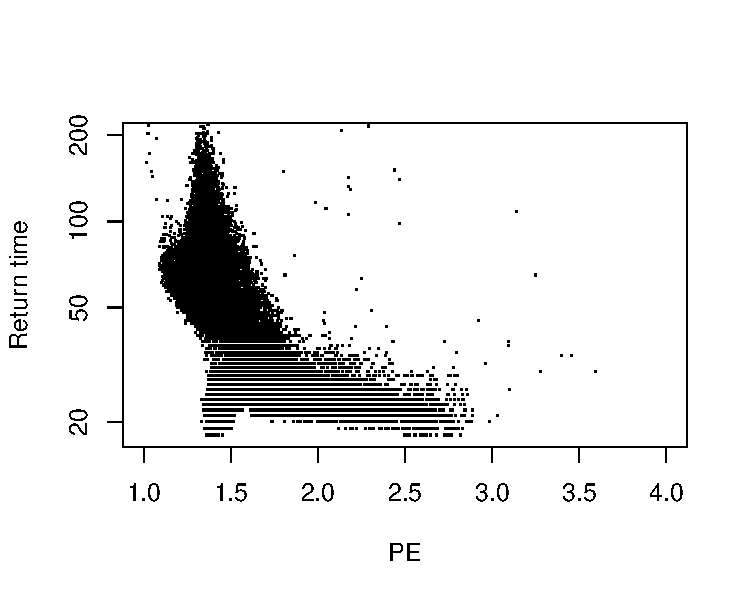
\includegraphics[width=0.5\textwidth]{figs2/fig_rtvspe.pdf}
\caption{
Return time vs. portfolio effect.
} \label{fig:rtvspe}
\end{figure}


% \begin{figure*}[h!]
%   \captionsetup{justification=raggedright,
% singlelinecheck=false
% }
% \centering
% \begin{subfigure}[t]{0.55\textwidth}
% \centering
% 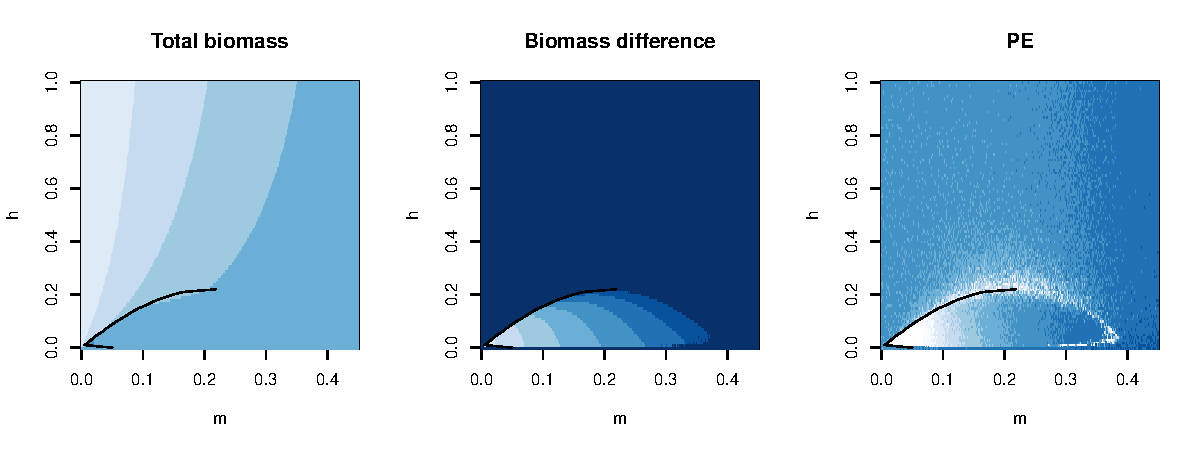
\includegraphics[width=\textwidth]{figs2/fig_MDPE_hm_theta3.pdf} 
% \caption{Low habitat heterogeneity ($\Delta\theta=3$)} \label{fig:thetadiff1}
% \end{subfigure}
% \begin{subfigure}[t]{0.55\textwidth}
% \centering
% 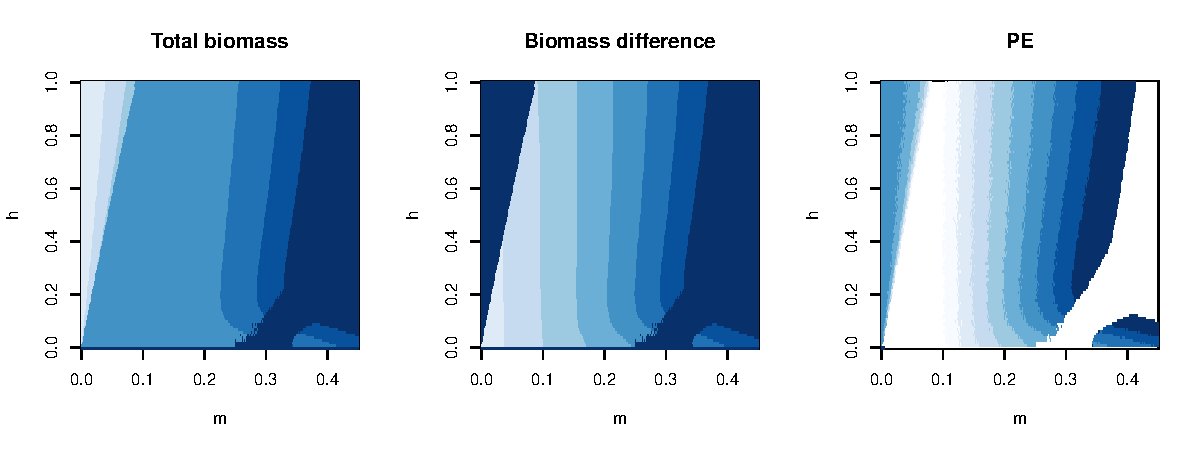
\includegraphics[width=\textwidth]{figs2/fig_MDPE_hm_theta8.pdf} 
% \caption{High habitat heterogeneity ($\Delta\theta=8$)} \label{fig:thetadiff2}
% \end{subfigure}
% \caption{Total means $N_t$, difference in means $\Delta N$, and the portfolio effect PE for different habitat heterogeneities $\Delta\theta$. Light colors = high values.
% }
% \end{figure*}


% \begin{figure*}[h!]
%   \captionsetup{justification=raggedright,
% singlelinecheck=false
% }
% \centering
% 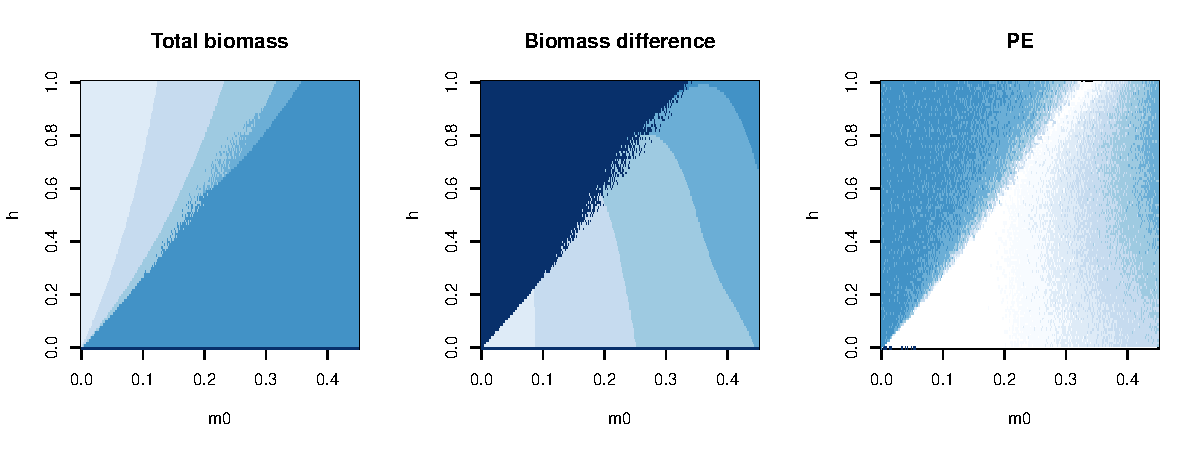
\includegraphics[width=0.8\textwidth]{figs2/fig_MDPE_hm_ddm.pdf}
% \caption{
% The same simulations as presented in Figure \ref{fig:PE}, except with density dependent straying, where $m(t) = m_0\left(1-N(t)/(C+N(t)\right)$. Light colors = high values.
% } \label{fig:ddm}
% \end{figure*}


\end{document}
